\documentclass[11pt]{article}
\title{Econ 103: Principle of Macroeconomics}
\author{Lanxiao Bai}
\date{\today}

\usepackage{amsmath}
\usepackage{tocloft}
\usepackage{graphicx}
\usepackage[bookmarks=true]{hyperref}

\renewcommand\cftdot{.}


\begin{document}
\maketitle
\newpage
\tableofcontents
\newpage

%Chapter 5
\section{Intro to Macroeconomics}
\subsection{Topics Macroeconomics concern}
    \begin{itemize}
        \item GDP
        \item Inflation
        \item Unemployment
    \end{itemize}
\subsection{Government role in economy}
    \begin{itemize}
        \item Fiscal policy 
        \item Monetary policy
        \item Growth policy
    \end{itemize}
\subsection{Category of Markets}
    \begin{itemize}
        \item Goods \& Service
        \item Money/Financial
        \item Labor
    \end{itemize}

%Chapter 6
\section{Measuring, National Output and income}
\subsection{GDP}
    \begin{itemize}
        \item Formula:
            \begin{equation}
                GDP = Aggregate expenditure=Aggregate income
            \end{equation}
        \item Definition: Production located \textbf{in the country}
        \item $Aggregate\ Expenditure = C + I + G + (EX - IM)$
        \begin{itemize}
            \item $C = Durable\ good + Nondurable\ good + service$
            \item $I = Residential\ Investment + Nonresidential\ Investment + Change\ in\ Inventories$
            \item $G = Government\ spending$
        \end{itemize}
        \item $Aggregate\ Income = national\ income + depreciation + (indirect\ taxes - subsidies) + net\ factor\ payments\ to\ the\ rest\ of\ the\ world + other$
    \end{itemize}
\subsection{GNP}
    Definition: Production owned by \textbf{a country’s citizen}

\subsection{Nominal and Real GDP}
\begin{itemize}
    \item $Nominal\ GDP = \sum Current\ Price\ \times Current\ production$
    \item $Real\ GDP = \sum {Base_year\ Price\ \times Current\ production}$
\end{itemize}

%Chapter 7
\section{Unemployment, Inflation, and Long-Run Growth}
\subsection{Ideal Economy}
    \begin{itemize}
        \item Low unemployment
        \item Low inflation
        \item Rapid growth of output
    \end{itemize}

\subsection{Feature of Labor Force and Categorize the Population}
    \subsubsection{Labor Force}
        Feature:
            \begin{itemize}
                \item Over 16 years old
                \item Have a job or is looking for a job
            \end{itemize}
        Unemployed:
            \begin{itemize}
                \item Is not working
                \item Is available for work
                \item Has effort to find a job
            \end{itemize}
    \subsubsection{Formulas}
    \begin{equation}
        Labor\ Force = Employed + Unemployed
    \end{equation}
    \begin{equation}
        People\ over\ 16 = In\ Labor\ Force + Not\ in\ Labor\ Force 
    \end{equation}
    \begin{equation}
        Unemployment\ Rate = \frac {Unemployed}{Labor\ Force}
    \end{equation}
    \begin{equation}
        Labor\ Force\ Participation\ Rate = \frac{Labor\ Force}{Population\ Over\ 16}
    \end{equation}
\subsection{Natural Unemployment}
    Natural Employmeny includes \textbf{Frictional Unemployment} and \textbf{Structral Unemployment}
    Definitions:
        \begin{itemize}
            \item Frictional Unemployment: Unemployment due to normal working of market like \textbf{Short-time Job/Skill Matching Problems}
            \item Structral Unemployment: Unemploymeny due to \textbf{Change of structure of ecomony}
        \end{itemize}

%Chapter 8
\section{Aggregate Expenditure \& Equilibrium Output without Govornment}
\subsection{Aggregate Income and GDP}
    \textbf{Formulas:}
    \begin{equation}
        Y\equiv C+S
    \end{equation}
    \begin{equation}
        C = a + MPC\cdot Y (0 < MPC < 1)
    \end{equation}
    \begin{equation}
        MPC + MPS = 1
    \end{equation}
    \begin{equation}
        Change\ in\ Inventory = Production - Sales
    \end{equation}
\subsection{Equilibrium}
    \begin{itemize}
        \item When equilibrium: $Y = AE \equiv C + I$
        \item When $Y > C + I$: Actual investment is greater than planned investment
        \item When $Y < C + I$: Actual investment is greater than planned investment
    \end{itemize}
\subsection{Mutiplier}
    \begin{equation}
        Multiplier = \frac{1}{MPS} = \frac{1}{1-MPC}
    \end{equation}
    \begin{equation}
        \Delta Y = \Delta I \times Multiplier
    \end{equation}

%Chapter 9
\section{Aggregate Expenditure \& Equilibrium Output with Government}
\subsection{Formulas}
After Tax Income:
\begin{equation}
    Y_d \equiv Y - T
\end{equation}
Aggregate Expenditure:
\begin{equation}
    AE \equiv C + I + G
\end{equation}
and
\begin{equation}
    C = a + MPC \times Y_d
\end{equation}
When equilibrium:
\begin{equation}
    Y = AE = C + I + G 
\end{equation}
Budget Deficit:
\begin{equation}
    D \equiv G - T
\end{equation}
\begin{equation}
    Leakages = Injections \Leftrightarrow S + T  = I + G
\end{equation}

\subsection{Multipliers}
    \begin{itemize}
        \item Government Spending Multiplier: $\frac{1}{MPS} = \frac{1}{1-MPC}$ and $\Delta Y = \frac{\Delta G}{MPS}$
        \item Tax Multiplier: $-\frac{MPC}{MPS}$ and $\Delta Y = \Delta T \cdot - \frac{MPC}{MPS}$
        \item Balanced Budget Multiplier: $1$ and $\Delta Y = \Delta G$
    \end{itemize}

%Chapter 10
\section{Money Supply and Federal Reserve System}
\subsection{Functions of Money}
    \begin{itemize}
        \item Means of Payment
        \item Storage of Value
        \item Unit of Account
    \end{itemize}
\subsection{Conceptions}
    \begin{itemize}
        \item Barter: Direct exchange of goods
        \item Commodity monies: Items used as money and also have \textbf{intrinsic value} in some other use
        \item Fiat / Token: Money that is \textbf{intrinsically worthless}
        \item Legal Tender: Money that govornment required to be accepted in settlement of debts
        \item M1(Transactions money): $=current\ held + demand\ deposits + travelers’\ check + other\ checkable\ deposits$
        \item M2(Broad money): $M1 + savings + money\ market accounts + other\ near\ monies$
    \end{itemize}

\subsection{Modern Bank System}
\textbf{Principle}: $Asset - Liabilities = Net\ Worth$\\\\
\textbf{Components:}\\

    \begin{tabular}{| c | c |}
        \hline
            Asset & Liability\\
        \hline
            Reserves & Deposits\\
            Loans & Net Worth\\
        \hline
    \end{tabular}

\subsection{Creation of money}
\paragraph{Principle}
$Actual\ Reserves \times Money\ Multiplier = Deposits\ created\ in\ banking\ system$
\paragraph{Money Multiplier}
$= \frac{1}{Required\ Reserve\ Ratio}$
\paragraph{Methods}
\begin{itemize}
    \item Changing \textbf{Required Reserve Ratio}
    \item Changing \textbf{Discount Rate}(New borrowed money become part of the reserve)
    \item \textbf{Open market operation}: purchase and sale government securities in open market
\end{itemize}

%Chapter 11
\section{Money demand, the equilibrium interest rate and monetary policy}
\subsection{Factors that affect demand for money}
\paragraph{Transaction Motive}
People hold money to buy things they need
\paragraph{Speculative Motive}
Invest the money they have to get more money
\subsection{Relation between Interest Rate and Money Supply}
Interest Rate and Money Supply is negatively related\\
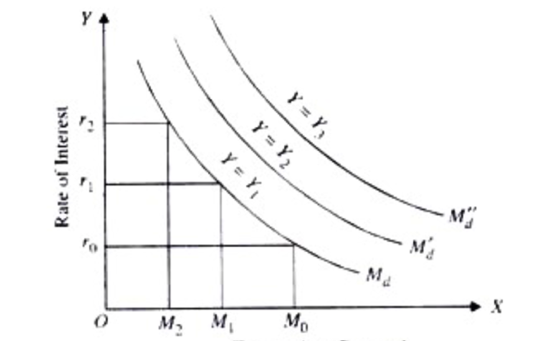
\includegraphics[width=10cm]{interest_rate.png}

\paragraph{Property}
\begin{itemize}
    \item $Y\uparrow \Rightarrow M^d \uparrow$(Shift Right)
    \item $Y\downarrow \Rightarrow M^d \downarrow$(Shift Left)
\paragraph{Money Demand and Supply Equilibrium}
The intercection point of MD and MS gives a point of equilibrium\\
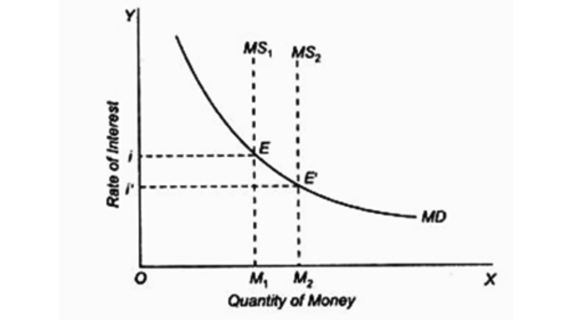
\includegraphics[width=10cm]{equilibrium.png}
\end{itemize}

\subsection{Monetary Policy}
\paragraph{Tight monetary policy}
Contract money supply to restrain the economy
\paragraph{Easy monetary policy}
Expand money supply to stimulate the ecomony

%Chapter 12
\section{Aggregate Demand in the Goods and Money Markets}
\subsection{How Goods Market and Money Market Related}
Goods Market: $Y = C + I + G$ ( depends on r)\\
Money Market: $M^d = M^s$ (Money demand depends on Y)
\begin{itemize}
    \item $Y\uparrow \Rightarrow M^d\uparrow \Rightarrow r\uparrow$
    \item $r\uparrow \Rightarrow I\downarrow \Rightarrow AE\downarrow \Rightarrow Y\downarrow$
\end{itemize}

\subsection{Effects of policies}
Expansionary fiscal policy(Crowd-out Effect):
\begin{equation}
    G\uparrow or\ T\downarrow \Rightarrow Y\uparrow \Rightarrow M^d\uparrow \Rightarrow r\uparrow \Rightarrow I\downarrow
\end{equation}
Expansionary Monetary Policy:
\begin{equation}
    M^s\uparrow \Rightarrow r\downarrow \Rightarrow I\uparrow \Rightarrow Y\uparrow \Rightarrow Y\uparrow \Rightarrow M^d \uparrow
\end{equation}
Contractionary fiscal policy:
\begin{equation}
    G\downarrow or\ T\uparrow \Rightarrow Y\downarrow \Rightarrow M^d\downarrow \Rightarrow r\downarrow \Rightarrow I\uparrow
\end{equation}
Contractionary monetary policy: 
\begin{equation}
    M^s\downarrow \Rightarrow r\uparrow \Rightarrow I\downarrow \Rightarrow Y\downarrow \Rightarrow Y\downarrow \Rightarrow M^d \downarrow
\end{equation}
Aggregate Demand (AD) curve: The higher the price level (P), the lower the aggregate e output, increase  , increase G or decrease T supply shift AD curve to the RIGHT, vice versa

%Chapter 13
\section{Aggregate Supply and the Equilibrium Price Level}
\subsection{Aggregate Supply Curve}
In the short run: $Y\uparrow \Rightarrow P\uparrow$
and
in the long run: AS curve is a vertical line, Y increase at the same rate as overall price level\\
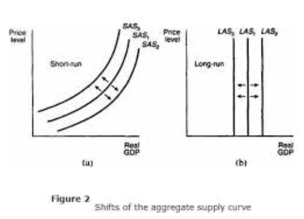
\includegraphics[width=10cm]{aggregate.png}
\subsection{Cost Shock on Supply}
\paragraph{Increase AS(shift right)}
    \begin{itemize}
        \item Lower cost
        \item Economic growth
        \item Public policy like tax cut, deregulation
        \item Good weather
    \end{itemize}
    
\paragraph{Decrease AS(shift left)}
    \begin{itemize}
        \item Higher cost
        \item Stagnation
        \item Public policy like waste, inefficiency and over-regulation
        \item Bad weather, disaster
    \end{itemize}
\subsection{Equilibrium}
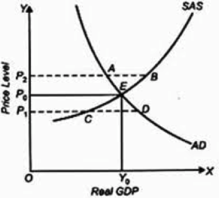
\includegraphics[width=10cm]{price_level.png}
%Chapter 14
\section{Labor Market}
\subsection{Classic View of Labor Market}
\subsubsection{Formulas}
\begin{equation}
        Labor\ Force = Employed + Unemployed
    \end{equation}
    \begin{equation}
        People\ over\ 16 = In\ Labor\ Force + Not\ in\ Labor\ Force 
    \end{equation}
    \begin{equation}
        Unemployment\ Rate = \frac {Unemployed}{Labor\ Force}
    \end{equation}
    \begin{equation}
        Labor\ Force\ Participation\ Rate = \frac{Labor\ Force}{Population\ Over\ 16}
    \end{equation}
    
    \subsubsection{Equilibrium}
    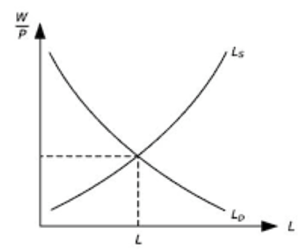
\includegraphics[width=10cm]{labor.png}
    
    Classical economists believe the labor market always clears because:
    \begin{itemize}
        \item When wage rates raise up, labor supply will increase
        \item Vice versa, when wage rates go down, people either accept job with lower wage or leave the job market

    \end{itemize}
\subsection{Beyond classical view}
    \subsubsection{Theories}
    \begin{itemize}
        \item Sticky wage (wage fails to fall when demand decrease)
        \item Social / implicit contract (unspoken agreement not to cut wage)
        \item Explicit contract (set wage explicitly)
        \begin{itemize}
            \item Cost of living adjustments (COLAs)
        \end{itemize}
        \item The efficiency wage theory
        \item Imperfect information (wrongly set wage due to lack of info)
        \item Minimum wage laws
    \end{itemize}
    \subsubsection{Philips Curve}
\textbf{Short-run Philips Curve}:\\

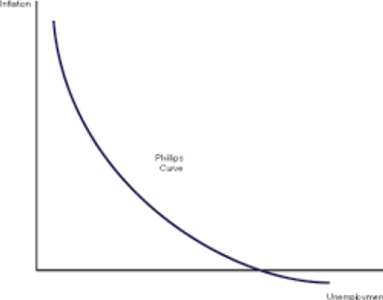
\includegraphics[width=10cm]{philips.png}

Phillips Curve fails to work in long run since both AD and AS are shifting and become vertical curve which intersect the x-axis at \textbf{Natural Rate of Unemployment} ($U^*$), which is at potential GDP.\\
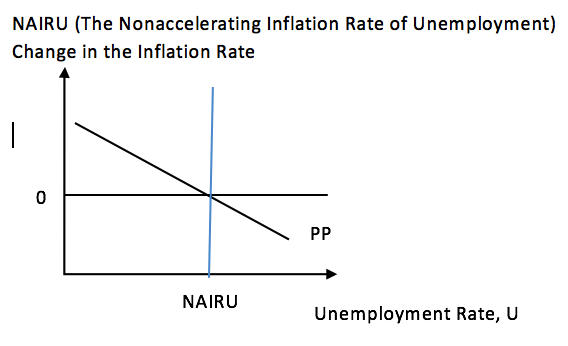
\includegraphics[width=10cm]{NAIRU.png}

Favorable shift is to the left, since we can have a lower NAIRU, which is caused by foreign competition
\begin{itemize}
    \item Input price$\uparrow\ \Rightarrow$ SPAS to the left, SRPC and PP to the right
    \item Inflationary expectation$\uparrow\ \Rightarrow$ SPAS to the left, SRPC and PP to the right
    \item Foreign Competition$\uparrow\ \Rightarrow$ SRAS to the right, SRPC and PP to the left
\end{itemize}

%Chapter 15
\section{Financial Crisis, Stabilization and Deficits}
\subsection{Methods to obtain money}
\begin{itemize}
    \item Bank Loan
    \item Bond issuance(Public debt)
    \item Stock(Ownership of a firm)
\end{itemize}
\subsection{Stock Market}
\paragraph{Factors that affect price of stock}
\begin{itemize}
\item Expectation of future profits
\item Expectation on what others would pay
\end{itemize}
\paragraph{Index to measure Stock Market}
\begin{itemize}
    \item Dow Jones Industrial(30)
    \item NASDAQ (Over 5000)
    \item Standard and Poor’s 500(500)
\end{itemize}
\subsection{Reasons for govornment's failure}
\paragraph{Time Lags}
\begin{itemize}
    \item Recognition Lag (Statistic)
    \item Implementation Lag (Congress)
    \item Response (Operation of economy itself)
\end{itemize}

Cut in government spending cause economy to contract, and decrease tax revenue, increase transfer payment

\subsection{Deficit Response Index (DRI)}
\paragraph{Method to calculate the effect of govornment action:}
\begin{enumerate}
    \item $\Delta Y = \Delta G \times Government\ Spending\ Multiplier$
    \item $\Delta D = \Delta Y \cdot DRI$
    \item $D = D_0 + \Delta D + \Delta G$
\end{enumerate}

%Chapter 17
\section{Long Run Growth}
\paragraph{Economic growth}
An increase in the total output of an economy

\paragraph{Factors}
\begin{itemize}
    \item Increase in Labor Supply
    \item Increase in physical or human capital
    \item Increase in Productivity
    \begin{itemize}
        \item Invention: Advance in knowledge
        \item Innovation: Use of new knowledge
    \end{itemize}
\end{itemize}

\paragraph{Limitations to growth}
\begin{itemize}
    \item Failure to enforce the rule of law
    \item Wars and revolutions
    \item Poor public health and education
    Law savings and investments
\end{itemize}

\paragraph{Policies for Faster Growth}
\begin{itemize}
    \item Stimulate Saving
    \item Stimulate Research and Developement
    \item Improve quality of education
    \item Improve health
    \item Encourage international education
\end{itemize}

%Chapter 18
\section{Alternative Views in Macroeconomics}
\subsection{Monetarism}
\paragraph{Velocity of Money}
$V \equiv \frac{GDP}{M}$
\paragraph{Nominal Income}
$GDP \equiv P \times Y$
$\Rightarrow  M \times V \equiv P \times Y$

\paragraph{Quantity Theory of Money}
Key assumption is that velocity of money is constant over time: $M \times \bar V = P \times Y$, which means that inflation is always and solely a monetary phenomenon. \textbf{Milton Friedman} advocated a policy of steady and slow money growth at the rate equal to the average growth of real output.

\subsection{New Classical Macroeconomics}
\subsubsection{Supply-Side Economics}
Supply-siders thinks that the problem of the economy is on supply side because of high rate of taxation abd heavy regulation that reduced the incentive to work, to save and to invest.

According to the Laffer Curve, there is some tax rate beyond which the supply response is large enough to lead to a decrease in tax revenue for further increase tax rate.

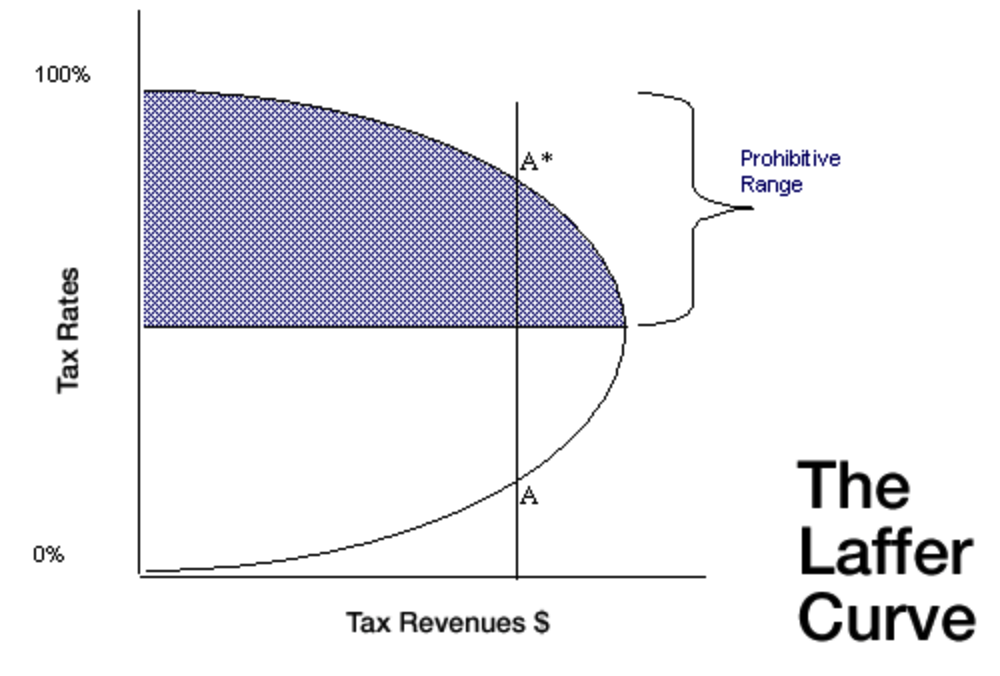
\includegraphics[width=10cm]{Laffer.png}

\subsection{New Keynesian Economics}
\paragraph{Assumption}
\begin{itemize}
    \item Rational Hypothesis
    \item Sticky Price
\end{itemize}

\paragraph{Lucas Supply Function}
$Y = f(P - P_{expect})$ embodies the idea that output depends on the differance between the actually price and expected price level.

%Chapter 19
\section{International Trade, Compatative Advantage and  Protectionism}
\subsection{International Trade}
\paragraph{Trade Surplus}
Export more than import
\paragraph{Trade Deficit}
Import more than export
\paragraph{David Ricardo's Theory of Comparative Advantage}
\begin{itemize}
    \item Absolute Advantage
    \item Comparative Advantage
    \item Specialization $\Rightarrow$ Mutual Benefit
\end{itemize}
\subsection{Other Theory and Concepts}
\paragraph{Terms of Trade}
The ratio at which a country can trade domestic products for imported products
\paragraph{Exchange Rate}
Ratio at which two currencies are traded, or the price of one currency in terms of another
\paragraph{Factor Endowments}
Quality and quantity of labor, land and natural resources of a country
\paragraph{Heckscher-Ohlin Theorem} A country has a comparative advantage in the production of a product if that country is relatively well endowed with inputs used intensively in the production of that product.
\subsection{Protectionism}
\paragraph{Protection}
A practice of shielding a sector of the economy from foreign competition
\paragraph{Tariff}
Tax on imports
\paragraph{Quota}
A limit on the quantity of imports
\paragraph{Dumping}
A industry that sells products in world market below the cost of production
\paragraph{Reason for protection}
\begin{itemize}
    \item Save jobs
    \item Fairness of competition
    \item National security
    \item Discourage dependency
    \item Protect infact industry
\end{itemize}
\subsection{Free Trade}
\begin{itemize}
    \item General Agreement on Tariff and Trade(GATT)
    \item World Trade Organization(WTO)
    \item European Union(EU)
    \item The North American Free-Trade Agreement(NAFTA)
\end{itemize}

%Chapter 20
\section{Open-economy macroeconomics}
\paragraph{Balance of payments}
Record of a country's transactions in goods, services and assets with the rest of the world and the supply and demand of foreign exchange
\paragraph{Current Account} The sum of:
\begin{itemize}
    \item Net Exports
    \item Net Income from investments abroad
    \item Net Transfer payments from abroad
\end{itemize}
\subsection{Equilibrium in an Open Economy}
\paragraph{Aggregate expenditure}
$AE \equiv C + I + G + EX - IM$
\begin{itemize}
    \item $C = a + bY$
    \item $I = I_0$
    \item $G = G_0$
    \item $EX = EX_0$
    \item $IM = mY$ 
\end{itemize}
$\Rightarrow Y^* = \frac{1}{1-b+m}(a+I+G+EX)$
\paragraph{Trade Feedback Effect}
The tendency for an increase in the economic activity of one country to lead to a worldwide increase in economic activity, which feeds back to that country. It is a process that \textbf{a domestic price increase in one country can "feed back" on itself through export and import prices}.

\subsection{Floating Exchange Rate}
In a money market where there is floating exchange rate, currency is like a good, and the equilibrium of its demand and supply determines its price.

\paragraph{The law of one price}
If the transportation fee is ignoreable, the price should be roughly the same

\paragraph{Effects of Exchange Rate on the Economy}
\begin{itemize}
    \item Depreciation: Increase spending on US goods $\Rightarrow$ AE increase $\Rightarrow$ Inventory fall $\Rightarrow$ GDP increase
    \item According to J Curve, the balance get worse before it gets better when depreciation 
\end{itemize}
    
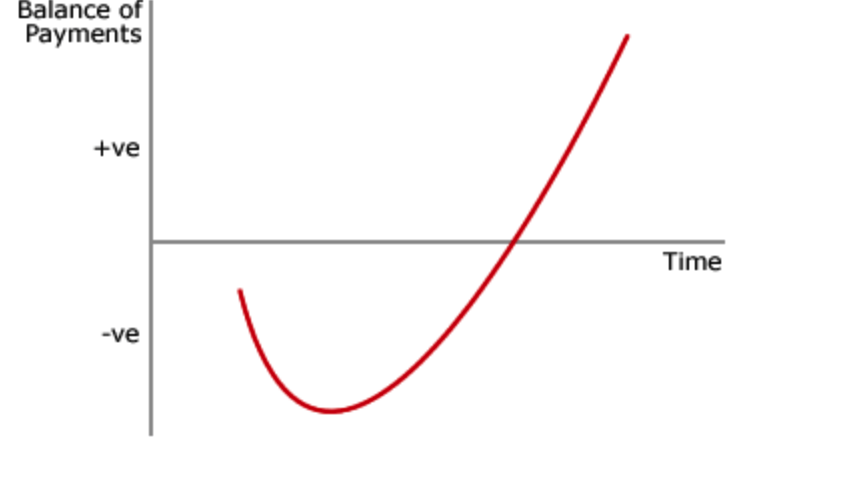
\includegraphics[width=10cm]{J.png}
\\\\\\\\\\\\\\\\\\\\
\centerline{END}
\end{document}
